% Introduction figure: what "dispersal" is, and the two currencies that pay
% for undoing it.  Conceptual schematic -- it plots no measured data, so it is
% built from this source rather than from the frozen registry.
%
% Build:  bash PaperDraft/scripts/build_intro_figure.sh
%
% Drawn in plain TikZ rather than quantikz: the object is a record *stream*
% with an annotated cut, not a gate circuit, and the cut/arrow geometry needs
% direct coordinate control.
%
% Scope discipline (see rem:round-contiguity, rem:dispersal in main.tex):
% the QAOA block is the in-scope example (contiguous rounds AND free per-round
% coefficients); the QPE ladder is drawn as the CONTRAST -- contiguous but
% coefficient-degenerate.  Neither is claimed as a theorem instance beyond
% what those remarks establish.
\documentclass[tikz,border=1pt]{standalone}
\usepackage{newtxtext,newtxmath}
\usepackage{amsmath}
\usetikzlibrary{arrows.meta,decorations.pathreplacing,calligraphy}

\definecolor{accent}{RGB}{28,86,140}
\definecolor{warn}{RGB}{150,60,40}
\definecolor{slab}{gray}{0.80}
\definecolor{faint}{gray}{0.92}

\begin{document}
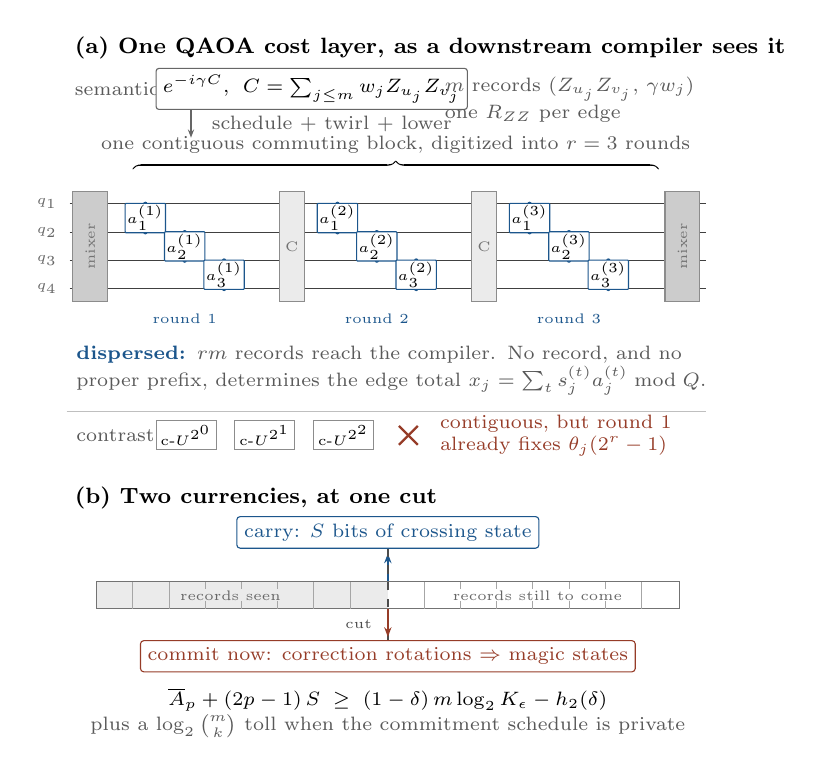
\begin{tikzpicture}[
  x=1cm,y=1cm,
  font=\footnotesize,
  wire/.style={line width=0.4pt,black!75},
  zzline/.style={line width=0.5pt,accent},
  dot/.style={circle,fill=accent,inner sep=0pt,minimum size=1.6pt},
  res/.style={draw=accent,line width=0.4pt,fill=white,inner sep=0.7pt,
              font=\tiny,rounded corners=0.3pt},
  slabbox/.style={draw=black!45,line width=0.4pt,fill=slab},
  cliff/.style={draw=black!45,line width=0.4pt,fill=faint},
  note/.style={font=\scriptsize,black!65},
  tag/.style={font=\tiny,black!60},
  panel/.style={font=\footnotesize\bfseries,black},
  callout/.style={draw,line width=0.4pt,fill=white,rounded corners=1.2pt,
                  inner sep=2.6pt,font=\scriptsize},
]

% ============================ PANEL (a) ============================
\node[panel,anchor=west] at (0,3.00)
  {(a) One QAOA cost layer, as a downstream compiler sees it};

% ---- semantic row ----
\node[note,anchor=west] at (0,2.48) {semantic};
\node[draw=black!60,line width=0.4pt,rounded corners=1pt,fill=white,
      inner sep=2.4pt,anchor=west,font=\scriptsize] at (1.15,2.48)
      {$e^{-i\gamma C}$,\; $C=\textstyle\sum_{j\le m} w_j Z_{u_j}Z_{v_j}$};
\node[note,anchor=west] at (4.70,2.48) {$m$ records $(Z_{u_j}Z_{v_j},\,\gamma w_j)$};
\node[note,anchor=west] at (4.70,2.16) {one $R_{ZZ}$ per edge};

% ---- lowering arrow ----
\draw[-{Stealth[length=3pt]},line width=0.5pt,black!60] (1.60,2.22) -- (1.60,1.86);
\node[note,anchor=west] at (1.74,2.04) {schedule $+$ twirl $+$ lower};

% ---- brace over the contiguous block ----
\node[note,anchor=south] at (4.20,1.54)
      {one contiguous commuting block, digitized into $r=3$ rounds};
\draw[decorate,decoration={calligraphic brace,amplitude=3pt},
      line width=0.5pt,black!55] (0.86,1.46) -- (7.54,1.46);

% ---- dispersed circuit row ----
% NB: not \wa..\wd -- \wd is a TeX primitive (box width).
\def\qA{1.02}\def\qB{0.66}\def\qC{0.30}\def\qD{-0.06}
\foreach \y in {\qA,\qB,\qC,\qD}{\draw[wire] (0.06,\y) -- (8.14,\y);}
\node[tag,anchor=east] at (0.02,1.02) {$q_1$};
\node[tag,anchor=east] at (0.02,0.66) {$q_2$};
\node[tag,anchor=east] at (0.02,0.30) {$q_3$};
\node[tag,anchor=east] at (0.02,-0.06) {$q_4$};

% mixer slabs = block boundaries (non-Clifford R_X: outside Def. 16)
\foreach \x in {0.10,7.62}{
  \fill[slabbox] (\x,-0.22) rectangle (\x+0.44,1.18);
  \node[rotate=90,font=\tiny,black!55] at (\x+0.22,0.48) {mixer};
}

% Clifford records between rounds (inside Def. 16 via lem:clifford-interleaving)
\foreach \x in {2.72,5.16}{
  \fill[cliff] (\x,-0.22) rectangle (\x+0.32,1.18);
  \node[font=\tiny,black!55] at (\x+0.16,0.48) {C};
}

% three contiguous rounds, three ZZ couplings each
\foreach \x/\t in {1.02/1,3.46/2,5.90/3}{
  \foreach \dx/\ya/\yb/\j in {0.00/\qA/\qB/1, 0.50/\qB/\qC/2, 1.00/\qC/\qD/3}{
    \draw[zzline] (\x+\dx,\ya) -- (\x+\dx,\yb);
    \node[dot] at (\x+\dx,\ya) {};
    \node[dot] at (\x+\dx,\yb) {};
    \node[res] at (\x+\dx,{(\ya+\yb)/2}) {$a^{(\t)}_\j$};
  }
  \node[font=\tiny,accent] at (\x+0.50,-0.44) {round \t};
}

\node[note,anchor=north west,text width=8.1cm,align=left] at (0.02,-0.66)
  {\textcolor{accent}{\textbf{dispersed:}} $rm$ records reach the compiler.
   No record, and no proper prefix, determines the edge total
   $x_j=\sum_{t}s^{(t)}_j a^{(t)}_j \bmod Q$.};

% ---- contrast strip: the QPE ladder ----
\draw[black!25,line width=0.3pt] (0.02,-1.62) -- (8.14,-1.62);
\node[note,anchor=west] at (0.02,-1.92) {contrast};
\foreach \x/\k in {1.15/0,2.15/1,3.15/2}{
  \node[draw=black!45,line width=0.4pt,fill=white,inner sep=1.6pt,
        font=\tiny,anchor=west] at (\x,-1.92) {c-$U^{2^{\k}}$};
}
\draw[warn,line width=0.8pt] (4.24,-1.80) -- (4.48,-2.04);
\draw[warn,line width=0.8pt] (4.48,-1.80) -- (4.24,-2.04);
\node[note,anchor=west,text width=3.5cm,align=left] at (4.64,-1.92)
  {\textcolor{warn}{contiguous, but round 1 already fixes $\theta_j(2^r-1)$}};

% ============================ PANEL (b) ============================
\node[panel,anchor=west] at (0,-2.72) {(b) Two currencies, at one cut};

% carry callout (above the stream)
\node[callout,draw=accent,text=accent,anchor=south] at (4.10,-3.36)
      {carry: $S$ bits of crossing state};
\draw[-{Stealth[length=3.5pt]},line width=0.6pt,accent] (4.10,-3.78) -- (4.10,-3.42);

% record stream band
\fill[faint] (0.40,-4.12) rectangle (4.10,-3.78);
\draw[black!55,line width=0.4pt] (0.40,-4.12) rectangle (7.80,-3.78);
\foreach \x in {0.86,1.32,1.78,2.24,2.70,3.16,3.62,4.56,5.02,5.48,5.94,6.40,6.86,7.32}{
  \draw[black!35,line width=0.3pt] (\x,-4.12) -- (\x,-3.78);
}
\node[tag,fill=faint,inner sep=0.5pt] at (2.10,-3.95) {records seen};
\node[tag,fill=white,inner sep=0.5pt] at (6.00,-3.95) {records still to come};

% the cut
\draw[dashed,line width=0.6pt,black!70] (4.10,-4.52) -- (4.10,-3.30);
\node[tag,black!70,anchor=east] at (4.02,-4.32) {cut};

% commit callout (below the stream)
\draw[-{Stealth[length=3.5pt]},line width=0.6pt,warn] (4.10,-4.12) -- (4.10,-4.48);
\node[callout,draw=warn,text=warn,anchor=north] at (4.10,-4.52)
      {commit now: correction rotations $\Rightarrow$ magic states};

% the frontier, and the toll
\node[anchor=north,font=\scriptsize] at (4.10,-5.00)
  {$\overline A_p+(2p-1)\,S\;\ge\;(1-\delta)\,m\log_2 K_\epsilon-h_2(\delta)$};
\node[note,anchor=north] at (4.10,-5.34)
  {plus a $\log_2\binom{m}{k}$ toll when the commitment schedule is private};

\end{tikzpicture}
\end{document}
